\section*{6.8}
%\addcontentsline{toc}{section}{Question 1}

a) On pose les conditions suivantes selon le problème :
\begin{align*}
    m = 1,\ k=100,\ b = 0,\ y(0)=0,\ y'(0)=0,\ f(t) = 36\cos(8t)
\end{align*}

L'ÉDO à résoudre est :
\begin{align*}
    y''+100y=36\cos(8t)
\end{align*}

On prend la transformée de Laplace des deux bords de l'équation :
\begin{align*}
    \lap{\prt{y'' +100y}} &= 36 \lap{\prt{\cos(8t)}}\\
    s^2Y -sy(0)-y'(0)+100Y &= 36\cdot \f{s}{s^2+8^2}\\
    Y(s^2+10^2) &= 36\cdot \f{s}{s^2+8^2}\\
    Y &= \f{36s}{(s^2+10^2)(s^2+8^2)}
\end{align*}

On utilise la fonction expand de la Ti sur l'expression précédente pour obtenir
le résultat suivant :
\begin{align*}
    Y = \f{s}{s^2+8^2}- \f{s}{s^2+10^2}
\end{align*}

On prend la transformée inverse en utilisant les tables de transformées. On
obtient alors :
\begin{align*}
    \ilap{\prt{Y}} = y(t) &= \ilap{\prt{\f{s}{s^2+8^2}-\f{s}{s^2+10^2}}}\\
    y(t) &= \cos(8t)-\cos(10t)
\end{align*}

Soit l'identité trigonométrique suivante :
\begin{align*}
    2\sin(\theta)\sin(\phi) = \cos(\theta - \phi)-\cos(\theta + \phi)
\end{align*}

Si on pose :
\begin{align*}
    \theta = t,\ \phi = 9t
\end{align*}

alors :
\begin{align*}
    2\sin(t)\sin(9t) &= \cos(t-9t)-\cos(t+9t)\\
    &= \cos(-8t)-\cos(10t)\\
    &= \cos(8t)-\cos(10t)\\
    2\sin(t)\sin(9t) &= y(t)
\end{align*}

b) Voici le graphique de $y(t)$ :
\begin{center}
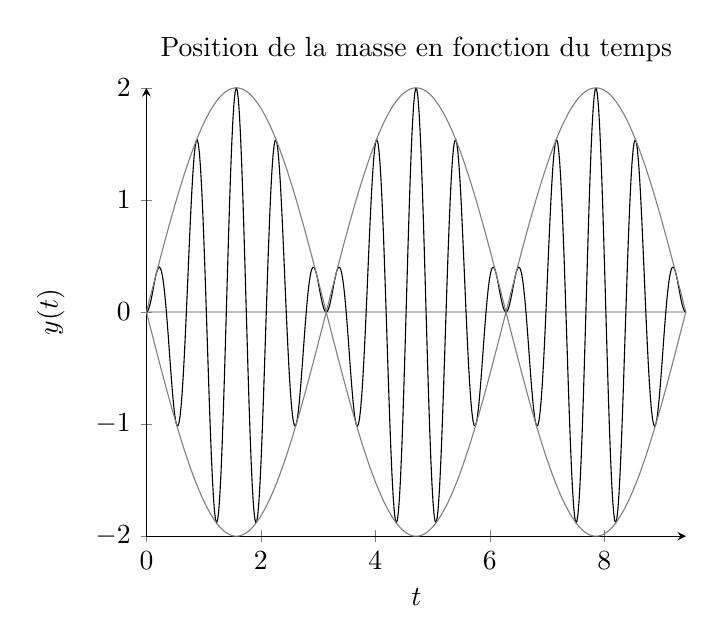
\begin{tikzpicture}
\begin{axis}[
    title = Position de la masse en fonction du temps,
    extra y ticks       = 0,
    extra y tick labels = ,
    extra y tick style  = { grid = major },
    axis lines = left,
    xlabel = \(t\),
    ylabel = {\(y(t)\)},
]
% Plot de la position
\addplot [
    domain=0:9.43, 
    samples=500, 
    color=black,
] {2*sin(deg(x))*sin(deg(9*x))};

\addplot [
    domain=0:9.43, 
    samples=500, 
    color=gray,
] {2*sin(deg(x))};

\addplot [
    domain=0:9.43, 
    samples=500, 
    color=gray,
] {-2*sin(deg(x))};
\end{axis}
\end{tikzpicture}
\end{center}
